\documentclass{standalone}
\usepackage{tikz}
\usetikzlibrary{calc,arrows.meta,decorations.markings,math,patterns}
\ifpdftex\usepackage[scaled=1]{helvet}\fi
\ifxetex\usepackage{fontspec}\setsansfont{TeX Gyre Heros}\fi
\begin{document}
\begingroup
\ifpdftex
\renewcommand\sfdefault{phv}
\renewcommand\rmdefault{phv}
\renewcommand\ttdefault{pcr}
\fi
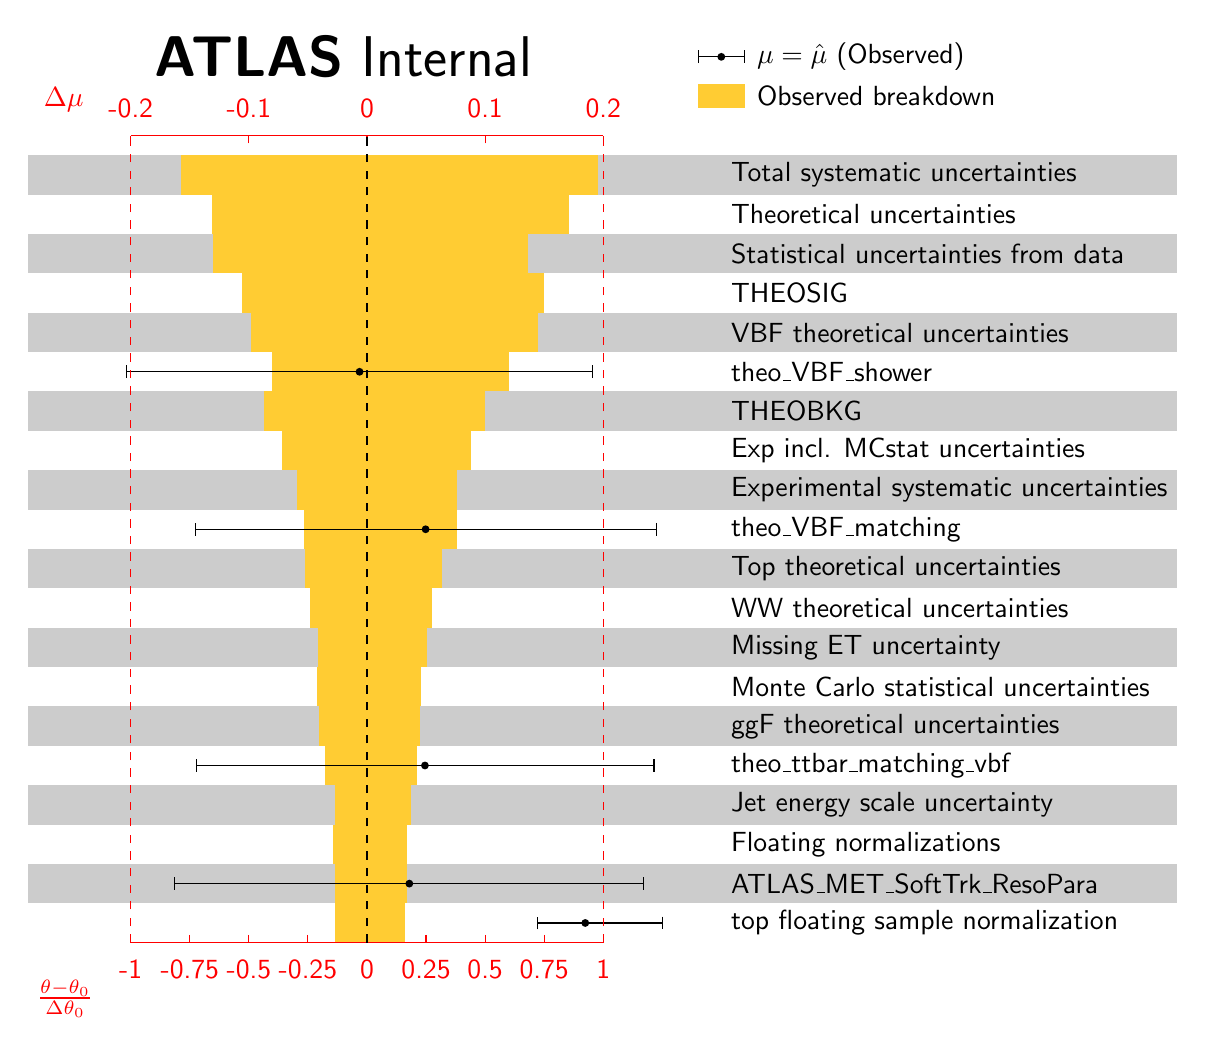
\begin{tikzpicture}[x=3cm,y=.5cm,%
  axlbl/.style={scale=1,anchor=center},%
  pull/.style={{|[scale=1]}-{|[scale=1]}},%
  dot/.style={circle,fill,inner sep=1pt,scale=1},
  every node/.append style={font=\sffamily}
]

  % defining the new dimensions and parameters
\newlength{\hatchspread}
\newlength{\hatchthickness}
\newlength{\hatchshift}
\newcommand{\hatchcolor}{}
% declaring the keys in tikz
\tikzset{hatchspread/.code={\setlength{\hatchspread}{#1}},
         hatchthickness/.code={\setlength{\hatchthickness}{#1}},
         hatchshift/.code={\setlength{\hatchshift}{#1}},% must be >= 0
         hatchcolor/.code={\renewcommand{\hatchcolor}{#1}}}
% setting the default values
\tikzset{hatchspread=3pt,
         hatchthickness=0.4pt,
         hatchshift=0pt,% must be >= 0
         hatchcolor=black}
% declaring the pattern
\pgfdeclarepatternformonly[\hatchspread,\hatchthickness,\hatchshift,\hatchcolor]% variables
   {custom north west lines}% name
   {\pgfqpoint{\dimexpr-2\hatchthickness}{\dimexpr-2\hatchthickness}}% lower left corner
   {\pgfqpoint{\dimexpr\hatchspread+2\hatchthickness}{\dimexpr\hatchspread+2\hatchthickness}}% upper right corner
   {\pgfqpoint{\dimexpr\hatchspread}{\dimexpr\hatchspread}}% tile size
   {% shape description
    \pgfsetlinewidth{\hatchthickness}
    \pgfpathmoveto{\pgfqpoint{0pt}{\dimexpr\hatchspread+\hatchshift}}
    \pgfpathlineto{\pgfqpoint{\dimexpr\hatchspread+0.15pt+\hatchshift}{-0.15pt}}
    \ifdim \hatchshift > 0pt
      \pgfpathmoveto{\pgfqpoint{0pt}{\hatchshift}}
      \pgfpathlineto{\pgfqpoint{\dimexpr0.15pt+\hatchshift}{-0.15pt}}
    \fi
    \pgfsetstrokecolor{\hatchcolor}
    \pgfusepath{stroke}
   }
  
\definecolor{colOverlay.Ranking.BREAKDOWNPos}{rgb}{1.000000,0.800000,0.200000}
\definecolor{colOverlay.Ranking.BREAKDOWNNeg}{rgb}{1.000000,0.800000,0.200000}
\definecolor{colOverlay.Ranking.BREAKDOWNHatchPos}{rgb}{1.000000,0.800000,0.200000}
\definecolor{colOverlay.Ranking.BREAKDOWNHatchNeg}{rgb}{1.000000,0.800000,0.200000}
\tikzset{Overlay.Ranking.BREAKDOWNPos/.style={draw=none,fill=colOverlay.Ranking.BREAKDOWNPos,text opacity = 1.0, fill opacity=1,}}
\tikzset{Overlay.Ranking.BREAKDOWNNeg/.style={draw=none,fill=colOverlay.Ranking.BREAKDOWNNeg,text opacity = 1.0, fill opacity=1,}}
\definecolor{colEffectAxes}{rgb}{1.000000,0.000000,0.000000}
\definecolor{colOverlay.Pulls.PULLS.observed}{rgb}{0.000000,0.000000,0.000000}
\tikzset{Overlay.Pulls.PULLS.observed/.style={pull,color=colOverlay.Pulls.PULLS.observed}}
\definecolor{colPullAxes}{rgb}{1.000000,0.000000,0.000000}
\definecolor{colHighlighting}{rgb}{0.800000,0.800000,0.800000}
\node[scale=1.,align=left] at (-0.1,2) {\huge\textbf{ATLAS} Internal};
\begin{scope}[name=legend,shift={(1.5,1)},x=0.3cm,y=.5cm]\draw[Overlay.Ranking.BREAKDOWNNeg](-1,-0.3) rectangle (0,0.3);
\draw[Overlay.Ranking.BREAKDOWNPos](0,-0.3) rectangle (1,0.3);
\node[anchor=west] at(1.1,0){Observed breakdown};
\draw[Overlay.Pulls.PULLS.observed](-1,1) -- (1,1);\node[dot,colOverlay.Pulls.PULLS.observed] at (0,1) {};
\node[anchor=west] at(1.1,1){$\mu = \hat{\mu}$ (Observed)};
\end{scope}\pgfdeclarelayer{background}\pgfsetlayers{background,main}
\node[scale=1,anchor=west,rotate=0] at (1.5,-1) {Total systematic uncertainties};
\node[scale=1,anchor=west,rotate=0] at (1.5,-2) {Theoretical uncertainties};
\node[scale=1,anchor=west,rotate=0] at (1.5,-3) {Statistical uncertainties from data};
\node[scale=1,anchor=west,rotate=0] at (1.5,-4) {THEOSIG};
\node[scale=1,anchor=west,rotate=0] at (1.5,-5) {VBF theoretical uncertainties};
\node[scale=1,anchor=west,rotate=0] at (1.5,-6) {theo\_VBF\_shower};
\node[scale=1,anchor=west,rotate=0] at (1.5,-7) {THEOBKG};
\node[scale=1,anchor=west,rotate=0] at (1.5,-8) {Exp incl. MCstat uncertainties};
\node[scale=1,anchor=west,rotate=0] at (1.5,-9) {Experimental systematic uncertainties};
\node[scale=1,anchor=west,rotate=0] at (1.5,-10) {theo\_VBF\_matching};
\node[scale=1,anchor=west,rotate=0] at (1.5,-11) {Top theoretical uncertainties};
\node[scale=1,anchor=west,rotate=0] at (1.5,-12) {WW theoretical uncertainties};
\node[scale=1,anchor=west,rotate=0] at (1.5,-13) {Missing ET uncertainty};
\node[scale=1,anchor=west,rotate=0] at (1.5,-14) {Monte Carlo statistical uncertainties};
\node[scale=1,anchor=west,rotate=0] at (1.5,-15) {ggF theoretical uncertainties};
\node[scale=1,anchor=west,rotate=0] at (1.5,-16) {theo\_ttbar\_matching\_vbf};
\node[scale=1,anchor=west,rotate=0] at (1.5,-17) {Jet energy scale uncertainty};
\node[scale=1,anchor=west,rotate=0] at (1.5,-18) {Floating normalizations};
\node[scale=1,anchor=west,rotate=0] at (1.5,-19) {ATLAS\_MET\_SoftTrk\_ResoPara};
\node[scale=1,anchor=west,rotate=0] at (1.5,-20) {top floating sample normalization};
\begin{scope}[name=ranking,colEffectAxes,xscale=5]
  \draw[Overlay.Ranking.BREAKDOWNNeg](-0.157541,-1.5) rectangle (0,-0.5);
  \draw[Overlay.Ranking.BREAKDOWNPos](0,-1.5) rectangle (0.195787,-0.5);
  \draw[Overlay.Ranking.BREAKDOWNNeg](-0.131041,-2.5) rectangle (0,-1.5);
  \draw[Overlay.Ranking.BREAKDOWNPos](0,-2.5) rectangle (0.170993,-1.5);
  \draw[Overlay.Ranking.BREAKDOWNNeg](-0.130531,-3.5) rectangle (0,-2.5);
  \draw[Overlay.Ranking.BREAKDOWNPos](0,-3.5) rectangle (0.136535,-2.5);
  \draw[Overlay.Ranking.BREAKDOWNNeg](-0.105684,-4.5) rectangle (0,-3.5);
  \draw[Overlay.Ranking.BREAKDOWNPos](0,-4.5) rectangle (0.150167,-3.5);
  \draw[Overlay.Ranking.BREAKDOWNNeg](-0.0978571,-5.5) rectangle (0,-4.5);
  \draw[Overlay.Ranking.BREAKDOWNPos](0,-5.5) rectangle (0.144695,-4.5);
  \draw[Overlay.Ranking.BREAKDOWNNeg](-0.0805606,-6.5) rectangle (0,-5.5);
  \draw[Overlay.Ranking.BREAKDOWNPos](0,-6.5) rectangle (0.120544,-5.5);
  \draw[Overlay.Ranking.BREAKDOWNNeg](-0.0870247,-7.5) rectangle (0,-6.5);
  \draw[Overlay.Ranking.BREAKDOWNPos](0,-7.5) rectangle (0.100067,-6.5);
  \draw[Overlay.Ranking.BREAKDOWNNeg](-0.0723303,-8.5) rectangle (0,-7.5);
  \draw[Overlay.Ranking.BREAKDOWNPos](0,-8.5) rectangle (0.0881595,-7.5);
  \draw[Overlay.Ranking.BREAKDOWNNeg](-0.0595601,-9.5) rectangle (0,-8.5);
  \draw[Overlay.Ranking.BREAKDOWNPos](0,-9.5) rectangle (0.076233,-8.5);
  \draw[Overlay.Ranking.BREAKDOWNNeg](-0.0531906,-10.5) rectangle (0,-9.5);
  \draw[Overlay.Ranking.BREAKDOWNPos](0,-10.5) rectangle (0.0764341,-9.5);
  \draw[Overlay.Ranking.BREAKDOWNNeg](-0.052659,-11.5) rectangle (0,-10.5);
  \draw[Overlay.Ranking.BREAKDOWNPos](0,-11.5) rectangle (0.063392,-10.5);
  \draw[Overlay.Ranking.BREAKDOWNNeg](-0.0483205,-12.5) rectangle (0,-11.5);
  \draw[Overlay.Ranking.BREAKDOWNPos](0,-12.5) rectangle (0.0548545,-11.5);
  \draw[Overlay.Ranking.BREAKDOWNNeg](-0.0413139,-13.5) rectangle (0,-12.5);
  \draw[Overlay.Ranking.BREAKDOWNPos](0,-13.5) rectangle (0.0504086,-12.5);
  \draw[Overlay.Ranking.BREAKDOWNNeg](-0.0427043,-14.5) rectangle (0,-13.5);
  \draw[Overlay.Ranking.BREAKDOWNPos](0,-14.5) rectangle (0.0457891,-13.5);
  \draw[Overlay.Ranking.BREAKDOWNNeg](-0.0403445,-15.5) rectangle (0,-14.5);
  \draw[Overlay.Ranking.BREAKDOWNPos](0,-15.5) rectangle (0.0451187,-14.5);
  \draw[Overlay.Ranking.BREAKDOWNNeg](-0.0357867,-16.5) rectangle (0,-15.5);
  \draw[Overlay.Ranking.BREAKDOWNPos](0,-16.5) rectangle (0.042283,-15.5);
  \draw[Overlay.Ranking.BREAKDOWNNeg](-0.0266858,-17.5) rectangle (0,-16.5);
  \draw[Overlay.Ranking.BREAKDOWNPos](0,-17.5) rectangle (0.0368555,-16.5);
  \draw[Overlay.Ranking.BREAKDOWNNeg](-0.0286778,-18.5) rectangle (0,-17.5);
  \draw[Overlay.Ranking.BREAKDOWNPos](0,-18.5) rectangle (0.0337934,-17.5);
  \draw[Overlay.Ranking.BREAKDOWNNeg](-0.0271009,-19.5) rectangle (0,-18.5);
  \draw[Overlay.Ranking.BREAKDOWNPos](0,-19.5) rectangle (0.0339361,-18.5);
  \draw[Overlay.Ranking.BREAKDOWNNeg](-0.0274609,-20.5) rectangle (0,-19.5);
  \draw[Overlay.Ranking.BREAKDOWNPos](0,-20.5) rectangle (0.0321753,-19.5);
  \draw (0,-0.2) -- (0,0) node [axlbl,above=3pt]{0};
  \draw (0.1,-0.2) -- (0.1,0) node [axlbl,above=3pt]{0.1};
  \draw (0.2,-0.2) -- (0.2,0) node [axlbl,above=3pt]{0.2};
  \draw (-0.1,-0.2) -- (-0.1,0) node [axlbl,above=3pt]{-0.1};
  \draw (-0.2,-0.2) -- (-0.2,0) node [axlbl,above=3pt]{-0.2};
  \draw (-0.2,0) -- (0.2,0);
  \node[axlbl,above left=5pt] at (-0.22,0) {$\Delta\mu$};
\end{scope}
\begin{scope}[name=pulls]
  \draw[Overlay.Pulls.PULLS.observed] (-1.02108,-6) -- (0.955567,-6);  \node[dot,colOverlay.Pulls.PULLS.observed] at (-0.031488,-6) {};
  \draw[Overlay.Pulls.PULLS.observed] (-0.729095,-10) -- (1.22681,-10);  \node[dot,colOverlay.Pulls.PULLS.observed] at (0.248246,-10) {};
  \draw[Overlay.Pulls.PULLS.observed] (-0.723311,-16) -- (1.21744,-16);  \node[dot,colOverlay.Pulls.PULLS.observed] at (0.24537,-16) {};
  \draw[Overlay.Pulls.PULLS.observed] (-0.815919,-19) -- (1.17462,-19);  \node[dot,colOverlay.Pulls.PULLS.observed] at (0.17932,-19) {};
  \draw[Overlay.Pulls.PULLS.observed] (0.717748,-20) -- (1.25411,-20);  \node[dot,colOverlay.Pulls.PULLS.observed] at (0.924059,-20) {};
\draw[colPullAxes] (-1,-20.3) -- (-1,-20.5) node [axlbl,below=3pt]{-1};
\draw[colPullAxes] (-0.75,-20.3) -- (-0.75,-20.5) node [axlbl,below=3pt]{-0.75};
\draw[colPullAxes] (-0.5,-20.3) -- (-0.5,-20.5) node [axlbl,below=3pt]{-0.5};
\draw[colPullAxes] (-0.25,-20.3) -- (-0.25,-20.5) node [axlbl,below=3pt]{-0.25};
\draw[colPullAxes] (0,-20.3) -- (0,-20.5) node [axlbl,below=3pt]{0};
\draw[colPullAxes] (0.25,-20.3) -- (0.25,-20.5) node [axlbl,below=3pt]{0.25};
\draw[colPullAxes] (0.5,-20.3) -- (0.5,-20.5) node [axlbl,below=3pt]{0.5};
\draw[colPullAxes] (0.75,-20.3) -- (0.75,-20.5) node [axlbl,below=3pt]{0.75};
\draw[colPullAxes] (1,-20.3) -- (1,-20.5) node [axlbl,below=3pt]{1};
\node[axlbl,colPullAxes,anchor=north east,xshift=-1em,yshift=-1em] at (-1,-20.5) {$\frac{\theta-\theta_0}{\Delta\theta_0}$};
\draw[colPullAxes] (-1,-20.5) -- (1,-20.5);
\draw[dashed,black] (0,-20.5) -- (0,0);
\draw[dashed,colPullAxes]   (-1,-20.5) -- (-1,0);
\draw[dashed,colPullAxes]   (1,-20.5) -- (1,0);
\end{scope}
\begin{pgfonlayer}{background}
  \foreach \i in {-1,-3,...,-20}{\fill[fill=colHighlighting] let \p1 = (current bounding box.east), \p2 = (current bounding box.west) in (\x1,\i-0.5) rectangle (\x2,\i+0.5); }
\end{pgfonlayer}
\end{tikzpicture}
\endgroup
\end{document}
